\documentclass[NET,english,beameralt]{tumbeamer}

\usepackage[utf8]{inputenc}
\usepackage{packages}
\usepackage{beamermods}
\usepackage{adjustbox}
\usepackage{attachfile}
\usepackage{fontawesome5}   % icons in the rendezvous diagram
\usepackage{bytefield}      % wire format on the backup slides
\usepackage{xurl}           % let long URLs in the bibliography break anywhere

% For beamer mode (default):
\author[D. Bachar]{Dan Bachar}
\title[Local Area P2P Overlays for Grassroots Social Networks]{Revisiting Local Area Peer-to-Peer Overlays\\ for Grassroots Social Networks}
\thesistype{final}{master}
\advisor{\unexpanded{David Guzman\\[0.5ex]Examiner: Prof.~Dr.-Ing.~J\"org Ott\\Supervisors: Prof.~Dr.~Idit Keidar, Prof.~Dr.~Ehud Shapiro}}
% TODO: confirm the defense date
\date{September 23, 2026}

% Narrow text columns look better ragged than justified: call \raggeditems inside the column
\newcommand{\raggeditems}{\renewcommand{\justify}{\raggedright}\raggedright}
% Ragged paragraph cells for tables
\newcolumntype{Y}[1]{>{\raggedright\arraybackslash}p{#1}}

% One-line message at the bottom of a results slide
\newcommand{\takeaway}[1]{\par\vspace{1.2ex}{\color{TUMBlue}\textbf{\(\Rightarrow\)\;#1}}\par}

% Timing plan for the 25-minute talk (the 5 minutes of questions follow; backup slides sit after the bibliography).
%   Title and five outline transitions   0:45
%   Introduction    4 frames             4:15
%   Background      4 frames             3:15
%   System design   6 frames             5:30
%   Evaluation      7 frames             8:15
%   Discussion, conclusion, future work  3:00
% The presenter script (talking points per frame, keyed by PDF page range) lives in
% speaker-script.txt next to this file, not in the LaTeX source. After editing the deck:
%   make && python3 pagemap.py --renumber speaker-script.txt

% byte offsets in the wire-format backup slide
\newcommand{\offset}[1]{\makebox[0pt][r]{#1 B\hspace{1.5em}}}

\usepackage{pgfpages}
\usepackage{ifthen}
% ============================================================================
% jobname solution
% ============================================================================
\newif\ifsolution%
\ifthenelse{\equal{\detokenize{notes}}{\jobname}}{%
\setbeameroption{show notes on second screen=bottom}
\setbeamercolor{note page}{bg=white, fg=black}
\setbeamercolor{note title}{bg=white!95!black, fg=black}
}{
}

% TeXLive 2018 compatibility: https://tex.stackexchange.com/questions/426088/texlive-pretest-2018-beamer-and-subfig-collide
\makeatletter
\let\@@magyar@captionfix\relax
\makeatother


\begin{document}
% Outline frame that highlights the current section: \outlineframe{<index>}
% 1 Introduction, 2 Background, 3 System Design, 4 Evaluation, 5 Conclusion, 6 Discussion
\newcommand{\outlineitem}[3]{%
    \ifnum#2<#1 \item {\color{TUMBlack}\large #3}\else
    \ifnum#2=#1 \item {\large\textbf{#3}}\else
    \item {\large #3}\fi\fi}
\newcommand{\outlineframe}[1]{%
\section{Outline}
\begin{frame}{}
    \vspace{1cm}
    \setbeamercolor{itemize/enumerate body}{fg=TUMBlue}
    \begin{itemize}
        \setlength\itemsep{1.4em}
        \setbeamertemplate{itemize item}{}
        \outlineitem{#1}{1}{Introduction}
        \outlineitem{#1}{2}{Background}
        \outlineitem{#1}{3}{System Design}
        \outlineitem{#1}{4}{Evaluation}
        \outlineitem{#1}{5}{Conclusion}
        \outlineitem{#1}{6}{Discussion}
    \end{itemize}
\end{frame}}

\section{Introduction}
\begin{frame}{Motivation}
    \begin{columns}[T]
    \column{1.0\textwidth}
    \raggeditems
    \begin{itemize}
        % \item Centralized platforms run on \emph{surveillance capitalism}: monetization of user data~\cite{Zuboff2023}
        % \item Internet shutdowns are a routine tool of \emph{networked autocracy}: governmental control of information, finance, media institutions~\cite{Lopez2026, Sarvestany2026, Bitchat-nepal, Bitchat-iran-uganda}
        % \item \emph{War and disasters} disrupt the physical network~\cite{gaza-brief,Aceto2026}
        \item Social networks that depend on any party but its members can be shut down.        
        \item Shutdowns, disasters, surveillance and control happen~\cite{Aceto2026,Lopez2026,Sarvestany2026,Zuboff2023}
        \item Use offline-first local communication, augmented with Internet instead of dependent on it
    \end{itemize}
    \end{columns}
    \vspace{2ex}
    \begin{columns}[T]
    \column{0.32\textwidth}
    \centering
    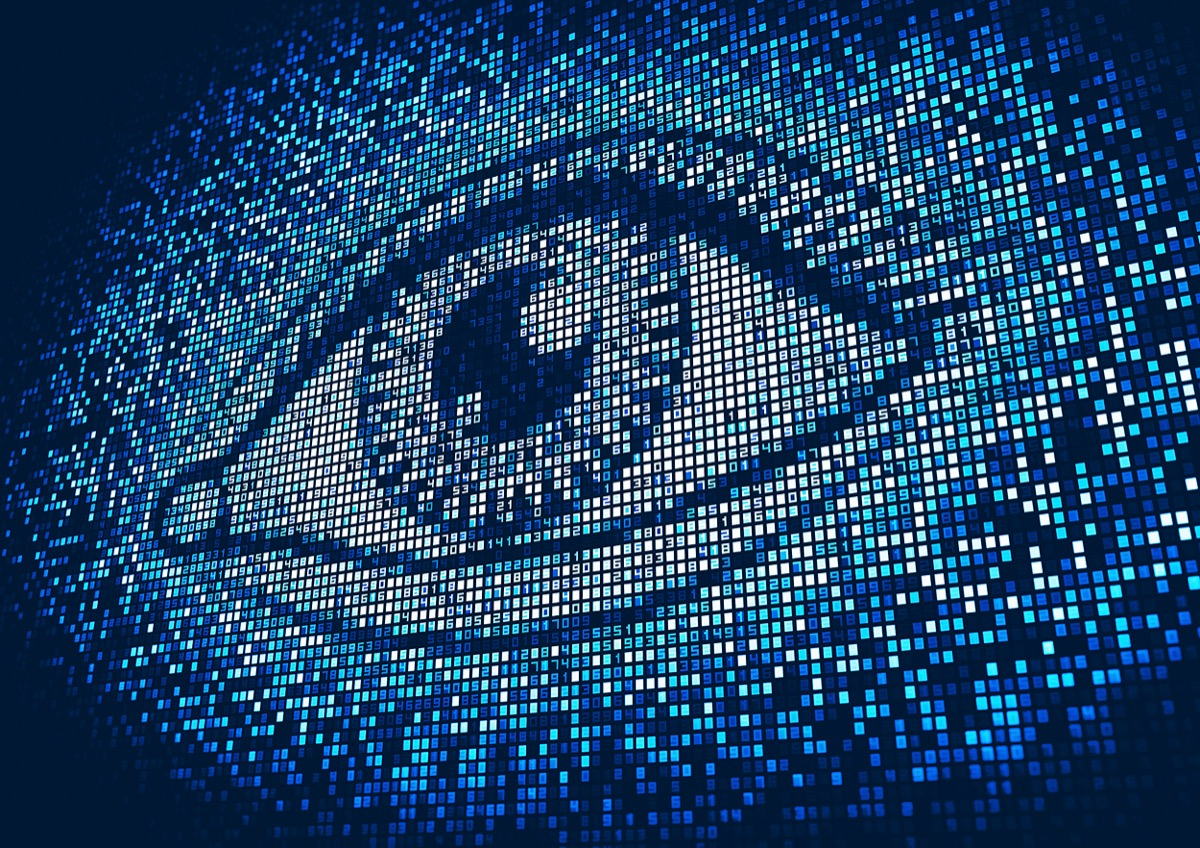
\includegraphics[height=2.1cm]{pics/surveillance-capitalism.jpg}\\{\tiny Harvard Gazette}
    \column{0.32\textwidth}
    \centering
    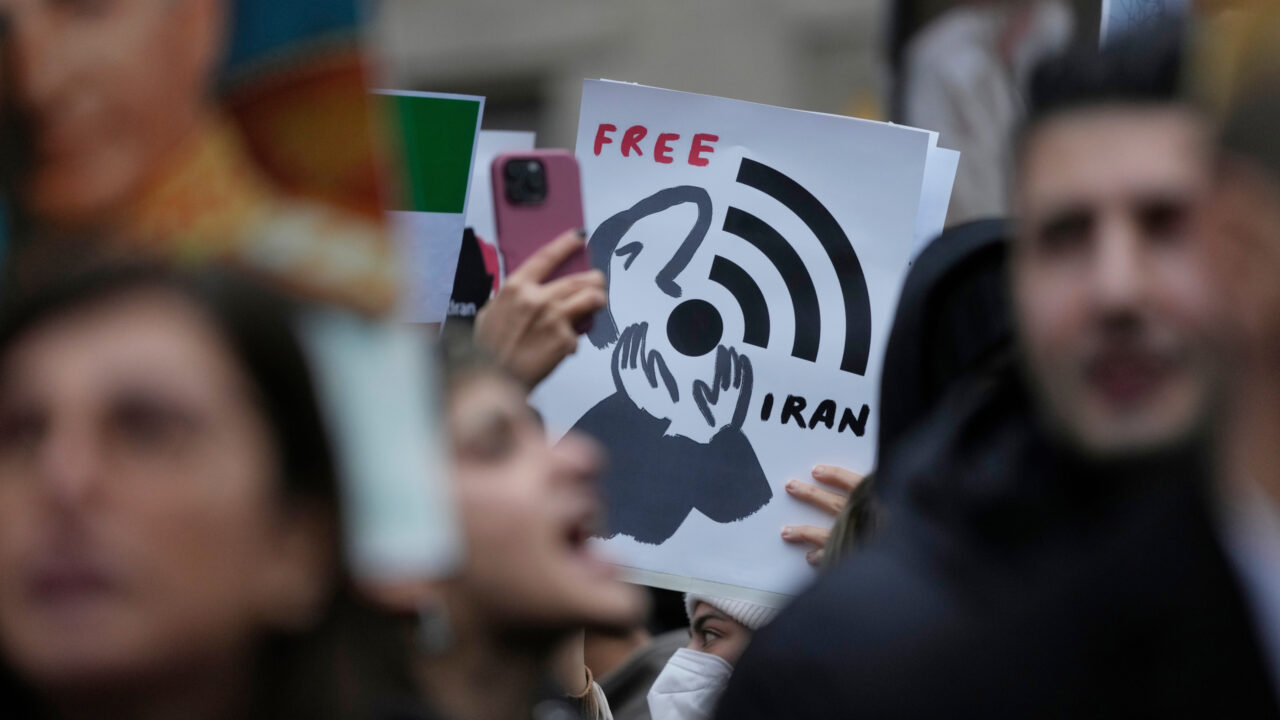
\includegraphics[height=2.1cm]{pics/networked-autocracy.jpg}\\{\tiny ECFR}
    \column{0.32\textwidth}
    \centering
    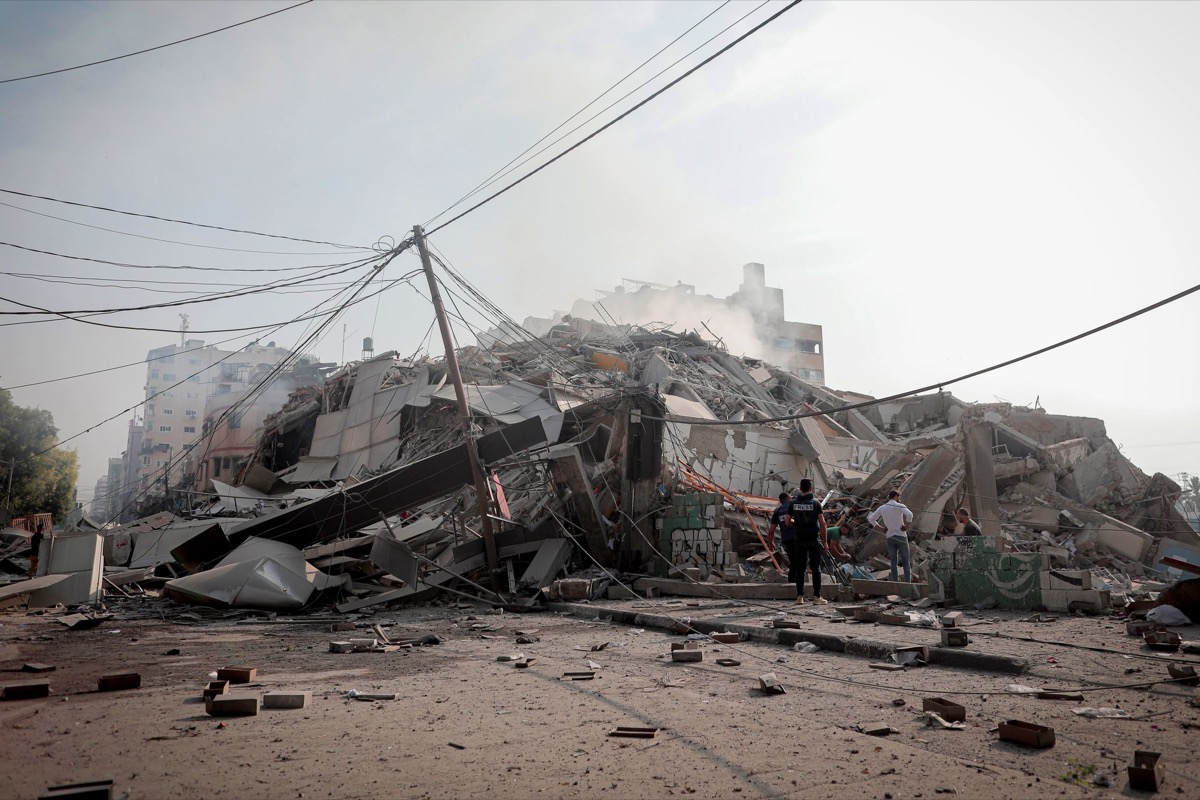
\includegraphics[height=2.1cm]{pics/gaza-outage.jpg}\\{\tiny Getty Images / WIRED}
    \end{columns}
\end{frame}
\begin{frame}{Problems}
    \noindent{\small$\Pi$ is every agent that could take part. A set $E\subseteq\Pi$ is \textbf{essential} if it is the minimal one whose removal leaves every remaining agent unable to interact with anyone; the smallest such $|E|$ sorts every platform into four classes~\cite[Def.~2.9,~2.10]{Shapiro2026Platforms}.}
    \par\vspace{0.5ex}
    \centering
    \small
    \setlength{\tabcolsep}{3pt}
    \begin{tabular}{@{}lY{1.7cm}Y{3.8cm}Y{2.7cm}@{}}
        \toprule
        Class & Example & Essential agents & cardinality \\
        \midrule
        Centralized & Facebook & the operator's own server~\cite{Lopez2026} & $|E|=1$ \\
        \midrule
        \multicolumn{4}{@{}l}{\emph{Distributed}~\cite{Jeong2025}} \\ \addlinespace[1.5ex]
        \quad Federated & Mastodon & \multirow{2}{=}{\raggedright instances, and bootstrap nodes: infinite, but not universal~\cite{Aravindh2019, Li2019}} &$|E|=\infty$, $|\Pi\setminus E|\ge 2$\\
        \quad Blockchain & Steemit & &$|E|=\infty$\\ \addlinespace[3ex]
        \quad Peer-to-peer & Briar, BitChat & Tor or Nostr relays~\cite{briar, bitchat} & $1<|E|<\infty$ \\
        \midrule
        \textbf{Grassroots} & \textbf{SSB, GNL} & \textbf{everyone}~\cite{Tarr2019, Shapiro2023} & $\Pi$\\
        \bottomrule
    \end{tabular}
    \par\vspace{0.5ex}
    \takeaway{A GSN has $|E|=\Pi\setminus\{p\}$: we chose to model our system after GSNs as universal set, having no central infrastructure}
\end{frame}

\begin{frame}{Background: OppNets}
    \begin{columns}[T]
    \column{0.56\textwidth}
    \raggeditems
    \begin{itemize}
        \item MANETs need a connected end-to-end path, which a crisis zone never offers~\cite{RFC2501, Conti2014}
        \item Opportunistic networks \emph{store, carry, forward} until a contact arises~\cite{Pelusi2006, RFC4838}
        \item Structured overlays give lower latency and a global state, but lean on designated nodes and degrade under churn~\cite{kademlia, chord, Lua2005}
        \item Unstructured overlays tolerate churn at the price of gossip overhead~\cite{Lua2005, guzman25}
        % \item Epidemic flooding delivers the most and congests first~\cite{Vahdat2000}
    \end{itemize}
    \column{0.42\textwidth}
    \centering
    \vspace{3mm}
    \begin{tikzpicture}[x=0.8mm,y=0.8mm, font=\scriptsize,
        dev/.style={circle, draw, thick, fill=white, minimum size=4.5mm, inner sep=0pt},
        lnk/.style={thick, TUMBlue}]
        \draw[dashed, black!50] (6,14) ellipse (11 and 12);
        \draw[dashed, black!50] (44,14) ellipse (11 and 12);
        \node[dev] (a1) at (1,14) {S};
        \node[dev] (a2) at (9,21) {};
        \node[dev] (a3) at (9,7) {};
        \draw[lnk] (a1)--(a2) (a1)--(a3) (a2)--(a3);
        \node[dev] (b1) at (49,14) {D};
        \node[dev] (b2) at (41,21) {};
        \node[dev] (b3) at (41,7) {};
        \draw[lnk] (b1)--(b2) (b1)--(b3) (b2)--(b3);
        \node[dev, fill=TUMOrange!30] (c) at (18,14) {C};
        \node[dev, fill=TUMOrange!30, dashed] (c2) at (32,14) {C};
        \draw[lnk, dashed] (a3)--(c);
        \draw[->, thick, TUMOrange] (c) -- (c2) node[midway, above] {carry};
        \draw[lnk, dashed] (c2)--(b3);
        \node[font=\scriptsize, TUMOrange, below=0.6mm of c] {store};
        \node[font=\scriptsize, TUMOrange, below=0.6mm of c2] {forward};
        \node[font=\scriptsize, black!60, align=center] at (25,-3) {no end-to-end path ever exists between S and D};
    \end{tikzpicture}
    \captionof{figure}{Store, carry, forward}
    \end{columns}
    \takeaway{Model GSN as OppNet with Store-carry-forward best effort delivery!}
\end{frame}

\begin{frame}{Solution Approach}
    \begin{moepdef}{blue}{filled}{Research question}
        What must be added to a BLE mesh, without introducing third party infrastructure, for a grassroots social network to deliver at scale?
    \end{moepdef}\par
    \vspace{1.5ex}
    \textbf{Contributions}
    \begin{itemize}
            % \item \textbf{Build} the networking layer: one application-layer overlay over a physical-layer local-area underlay and a transport-layer wide-area underlay
            \item \textbf{Measure} the grassroots networking layer on a testbed of commodity smartphones: what a link costs, how delivery degrades under contention, how often links flap
            \item \textbf{Simulate} at scale, calibrated on those measurements, to compare control-plane and forwarding strategies
            \item \textbf{Results} we found that contention collapses delivery even at close range, link outages are common on old hardware and heavy-tailed, and BLE-only saturates at 80\% delivery, with the Internet addition bridging to 100\%
    \end{itemize}
\end{frame}

\begin{frame}{Related Works}
    \begin{center}
    \small
    \setlength{\tabcolsep}{5pt}
    \begin{tabular}{@{}Y{2.2cm}Y{3.6cm}Y{2.6cm}Y{2.5cm}@{}}
        \toprule
        System & Local-area underlay & Wide-area underlay & Third-party dependency \\
        \midrule
        SSB~\cite{Tarr2019} & WLAN, Bluetooth Classic\textsuperscript{*} & pub servers over TCP&pub servers\\
        Briar~\cite{briar} & WLAN, Bluetooth Classic & Tor & Tor~\cite{Aceto2026} \\
        BitChat~\cite{bitchat} & BLE mesh & Nostr relays & the relays~\cite{Wei2025} \\
        Amigo~\cite{Inyangson2025} & Wi-Fi Direct & none & GPS \\
        % \midrule
        % \textbf{GNL} & BLE mesh, controlled flooding with custody & UDX streams between friends, NAT hole punching & none: friends act as rendezvous agents \\
        \bottomrule
    \end{tabular}
    \end{center}
    \begin{itemize}
        \item The component structure inherits from BitChat; Nostr relays replaced by edge rendezvous points (friends) for hole-punching
        % s\item Information travels along the edges of the social graph~\cite{Shapiro2023}
    \end{itemize}
\end{frame}

\outlineframe{2}
\section{Background}
\begin{frame}{The local-area underlay}
    \textbf{Six criteria}: interoperability and availability on commodity-grade smartphones, low power, works while backgrounded, tolerates mobility, needs no infrastructure, and carries a short message within a second~\cite{Nielsen1994}
    \begin{center}
    \small
    \setlength{\tabcolsep}{4pt}
    \begin{tabular}{@{}lcY{6.3cm}@{}}
        \toprule
        Technology & & Why \\
        \midrule
        Wi-Fi Ad-Hoc & \no & no power saving when idle~\cite{Friedman2013} \\
        Wi-Fi Direct, AirDrop, QuickShare & \no & requires a foreground app; no interoperability between iOS and Android~\cite{CampsMur2013} \\
        Wi-Fi Aware & \no & reached iOS only in 2025~\cite{Apple2025WWDC} \\
        Zigbee, LoRa, 6LoWPAN & \no & no device-to-device support on smartphones~\cite{Saloni2016} \\
        \textbf{Bluetooth Low Energy} & \yes & on all smartphones; duty-cycled radio; the OS advertises and scans in the background; about 200\,kb/s~\cite{Jacopo2017} \\
        \bottomrule
    \end{tabular}
    \end{center}
    % \vspace{0.5ex}
    % {\small BLE is the only technology that meets all six. Bluetooth 4.2's data length extension gives the 247-byte MTU the design builds on~\cite{TJonck2021}.}
\end{frame}

\begin{frame}{The wide-area underlay}
    % \textbf{For friends beyond radio range}: the transport must survive a change of network attachment point, and cost as little as possible to re-establish
    The transport must survive a change of network attachment point, and cost as little as possible to (re-)establish, no encryption or handshake
    \begin{center}
    \small
    \setlength{\tabcolsep}{4pt}
    \begin{tabular}{@{}lcY{6.6cm}@{}}
        \toprule
        Transport & & Why \\
        \midrule
        TCP & \no & the connection breaks when its 5-tuple changes, congestion control reads an outage as congestion~\cite{RFC9293, RFC5681}, and throughput falls with the hop count~\cite{Matei2002} \\
        Plain UDP & \no & survives address changes, but offers no reliability, ordering, or congestion control~\cite{RFC768} \\
        QUIC & \maybe & reliable and congestion-controlled, but pays a handshake and brings encryption the overlay already has~\cite{Langley2017} \\
        \textbf{UDX} & \yes & Similar to QUIC, but no handshake and no encryption~\cite{udx} \\
        \bottomrule
    \end{tabular}
    \end{center}
    \vspace{0.5ex}
    % {\small Noise supplies the security on top. NATs still drop unsolicited packets, so two friends need a signaling channel to punch a hole~\cite{RFC5128}.}
\end{frame}

\outlineframe{3}
\section{System Design}
\begin{frame}{One overlay, two underlays}
    \begin{columns}[T]
    \column{0.48\textwidth}
    \centering
    \begin{tikzpicture}[x=1mm,y=1mm, font=\footnotesize,
        box/.style={draw, thick, fill=white, align=center, inner sep=1.5pt},
        wide/.style={box, minimum width=54mm},
        half/.style={box, text width=25mm, minimum height=10mm},
        sub/.style={box, text width=15.5mm, minimum height=6mm, font=\scriptsize}]
        \node[wide, minimum height=6mm, fill=black!5] (app) at (27,50) {Grassroots Social Networks};
        \node[wide, minimum height=14mm, fill=TUMBlue!12] (gnl) at (27,37.5) {};
        \node[font=\footnotesize\bfseries] at (27,42.5) {GNL overlay};
        \node[sub] at (9.5,35) {Fragment and protocol handlers};
        \node[sub] at (27,35) {Noise session manager};
        \node[sub] at (44.5,35) {Message router, DTN buffer};
        \node[wide, minimum height=7mm, dashed, fill=black!3] (tsi) at (27,26) {Transport service interface};
        \node[half] (ble) at (13,14) {LAN PHY\\underlay adapter\\GATT links over BLE\\Mesh delivery};
        \node[half] (udp) at (41,14) {WAN Transport\\underlay adapter\\UDX streams over UDP\\direct delivery only};
        \node[half, minimum height=8mm, fill=black!5] (blephy) at (13,3) {OS BLE stack\\Central, Peripheral};
        \node[half, minimum height=8mm, fill=black!5] (ipphy) at (41,3) {OS UDP/IP stack\\Wi-Fi, Ethernet, cellular};
        \draw[->, thick] (app) -- (gnl);
        \draw[->, thick] (gnl) -- (tsi);
        \draw[->, thick] (tsi.south -| ble) -- (ble);
        \draw[->, thick] (tsi.south -| udp) -- (udp);
        \draw[->, thick] (ble) -- (blephy);
        \draw[->, thick] (udp) -- (ipphy);
    \end{tikzpicture}
    \captionof{figure}{GNL component architecture}
    \column{0.50\textwidth}
    \raggeditems
    \begin{itemize}
        \item GNL fragments to the path MTU, seals every fragment in the peer's Noise session, and picks the underlay that currently reaches the peer
        \item Radio first: a peer reachable over both is served over BLE
        \item No link to the recipient? The router takes custody and conveys the packet over the mesh
    \end{itemize}
    \end{columns}
\end{frame}

\begin{frame}{Identity, discovery, and trust}
    \centering
    \begin{tikzpicture}[x=1mm,y=1mm, font=\footnotesize]
        \node[draw, thick, fill=black!5, minimum width=50mm, minimum height=10mm, align=center] at (25,0) {\textbf{8 B fixed prefix}\\ \texttt{SHA-256("grassroots")}};
        \node[draw, thick, fill=TUMBlue!12, minimum width=66mm, minimum height=10mm, align=center] at (83,0) {\textbf{8 B rotating suffix}, new every 15 minutes\\ \texttt{SHA-256("grassroots ble suffix" | pubkey | slot)}};
    \end{tikzpicture}
    \captionof{figure}{The advertised BLE service UUID}
    \vspace{1ex}
    \begin{itemize}
        \item \textbf{Identity} is an Ed25519 key pair: the address, the signature, and the root of the session key
        \item \textbf{ANNOUNCE} broadcasts presence and identity
        \item Friends who know the key recognize the beacon; random to strangers and cannot be tracked across slots
        \item \textbf{Trust}: \emph{Closed} links only to friends and never relays; \emph{Open} links to any grassroots device and joins the mesh
    \end{itemize}
\end{frame}

\begin{frame}{Secure sessions and the packet header}
    \begin{itemize}
        \item \textbf{Noise XX} with \texttt{Curve25519} and \texttt{ChaCha20-Poly1305}~\cite{Kobeissi2018, polychacha}: a static key that differs from the announced one aborts the handshake
        \item One session per peer across both underlays, keyed by public key
        \item 60-byte outer envelope header with a recipient but \emph{no sender}: relays read only the \mbox{envelope}
        \item The receiver finds the sender by trial decryption against its sessions, to read inner encrypted envelope
        % \item The recipient field stays: without it every transit packet would be trial-decrypted, and 128 sessions saturate one Nexus 5X core at 22 packets per second
    \end{itemize}
\end{frame}

\begin{frame}{Routing over the BLE mesh}
    \begin{columns}[T]
    \column{0.54\textwidth}
    \raggeditems
    \begin{itemize}
        \item \textbf{Controlled flooding}: forward packets using GCS buffer reconciliation
        \item \textbf{Custody}: keep packets per recipient for 6 hours or until a delivery proof arrives
        \item \textbf{Fragmentation}: the 247-byte MTU leaves 138 B of payload per fragment~\cite{TJonck2021}
    \end{itemize}
    \column{0.44\textwidth}
    \centering
    \vspace{2mm}
    \begin{tikzpicture}[x=0.9mm,y=0.9mm, font=\footnotesize,
        dev/.style={circle, draw, thick, fill=white, minimum size=5.5mm, inner sep=0pt},
        hop/.style={->, thick, TUMBlue},
        ttl/.style={font=\scriptsize, fill=white, inner sep=1pt}]
        \node[dev] (s) at (0,16) {S};
        \node[dev] (a) at (16,28) {};
        \node[dev] (b) at (16,4) {};
        \node[dev] (c) at (32,16) {C};
        \node[dev] (e) at (32,38) {};
        \node[dev, dashed] (d) at (52,16) {D};
        \draw[hop] (s)--(a) node[ttl, midway] {TTL 7};
        \draw[hop] (s)--(b) node[ttl, midway] {TTL 7};
        \draw[hop] (a)--(c) node[ttl, midway] {6};
        \draw[hop] (b)--(c) node[ttl, midway] {6};
        \draw[hop] (a)--(e) node[ttl, midway] {6};
        \draw[hop, dashed] (c)--(d) node[ttl, midway] {5};
        \node[font=\scriptsize, black!60, align=center, text width=50mm] at (26,-9) {Duplicates are suppressed by packet ID. C keeps custody until it links with D or sees a delivery proof.};
    \end{tikzpicture}
    \captionof{figure}{Controlled flooding with custody}
    \end{columns}
\end{frame}

\begin{frame}{The IP path: rendezvous through friends}
    \begin{columns}[T]
    \column{0.42\textwidth}
    \centering
    \resizebox{\linewidth}{!}{
        \begin{tikzpicture}[
            smartphone_body/.style={
                draw, thick, rectangle, rounded corners=4pt,
                minimum width=0.8cm, minimum height=1.6cm, fill=white,
            },
            smartphone_screen/.style={draw, thick, rounded corners=1pt},
            smartphone_button/.style={draw, thick, circle},
            big_cloud/.style={
                draw, cloud, thick,
                minimum width=6cm, minimum height=3.8cm,
                cloud ignores aspect, cloud puffs=15,
                draw=gray!60
            },
            small_cloud/.style={
                draw, cloud, thick,
                minimum width=3.5cm, minimum height=2.5cm,
                cloud ignores aspect, cloud puffs=13,
                draw=gray!60
            },
            transition_arrow/.style={->, >=stealth, line width=2pt, draw=gray!60},
            lbl/.style={font=\Large\bfseries}
        ]
            % top: B is linked to A over BLE and to C over the Internet
            \node[big_cloud] (bigcloud) at (-3.5, 3.5) {};
            \node[smartphone_body] (pmain) at (-2.2, 4) {};
            \node[smartphone_body] (pleft_top) at (-4.8, 3) {};
            \node[smartphone_body] (pright_top) at (5, 3.5) {};
            \node[small_cloud] at (pright_top.center) {};
            \draw[thick] (pmain.center) -- (pleft_top.center)
                node[blue!70!black, fill=white, inner sep=2pt, midway] {\Large \faBluetoothB};
            \draw[thick] (pmain.center) -- (pright_top.center)
                node[green!40!black, fill=white, inner sep=2pt, midway] {\Large \faGlobe};
            \draw[transition_arrow] (0, 1.5) -- (0, 0.3);
            % bottom: A and C talk directly after the punch
            \node[smartphone_body] (p1_bot) at (-5, -1) {};
            \node[smartphone_body] (p2_bot) at (5, -1) {};
            \node[small_cloud] at (p1_bot.center) {};
            \node[small_cloud] at (p2_bot.center) {};
            \draw[thick] (p1_bot.center) -- (p2_bot.center)
                node[green!40!black, fill=white, inner sep=2pt] at (0, -1) {\Huge \faGlobe};
            \foreach \p in {pmain, pleft_top, pright_top, p1_bot, p2_bot} {
                \node[smartphone_body] at (\p) {};
                \draw[smartphone_screen] ($(\p)+(-0.3, -0.6)$) rectangle ($(\p)+(0.3, 0.7)$);
                \draw[smartphone_button] ($(\p)+(0,-0.5)$) circle (0.05cm);
            }
            \node[lbl, below=0.1cm of pleft_top] {A};
            \node[lbl, below=0.1cm of pmain] {B};
            \node[lbl, below=0.1cm of pright_top] {C};
            \node[lbl, below=0.1cm of p1_bot] {A};
            \node[lbl, below=0.1cm of p2_bot] {C};
        \end{tikzpicture}
    }
    \captionof{figure}{B, a mutual friend linked to A over BLE and to C over the Internet, signals the hole punch; afterwards A and C communicate directly}
    \column{0.56\textwidth}
    \raggeditems
    \begin{itemize}
        \item NATs drop unsolicited packets, so friends need a \emph{signaling channel} to punch holes~\cite{RFC5128}: a direct BLE link, or mutual online friends as rendezvous agents
        \item The rendezvous agent reflects each peer's public address and instructs both to send \texttt{punch} packets; signed \emph{friendship attestations} authorize it
        \item A UDX stream opens, then Noise XX authenticates it
        \item \textbf{Cold calls}: a signed, single-use invite link, valid for limited time
    \end{itemize}
    \end{columns}
\end{frame}

\outlineframe{4}
\section{Evaluation}
\begin{frame}{Testbed}
    \begin{itemize}
        \item Eight commodity smartphones on tripods, outdoors
        \item Every run traces RSSI, the time to each link stage, and bytes per packet class
        \item Messages are 138 B, the largest unfragmented payload
        \item Three experiments: the \emph{line} (distance), \emph{diluting clique} (contention), \emph{link flapping} (outages)
    \end{itemize}
\end{frame}

\begin{frame}{Experiment 1, the line: the path-loss fit}
    \begin{columns}[T]
    \column{0.55\textwidth}
    \centering
    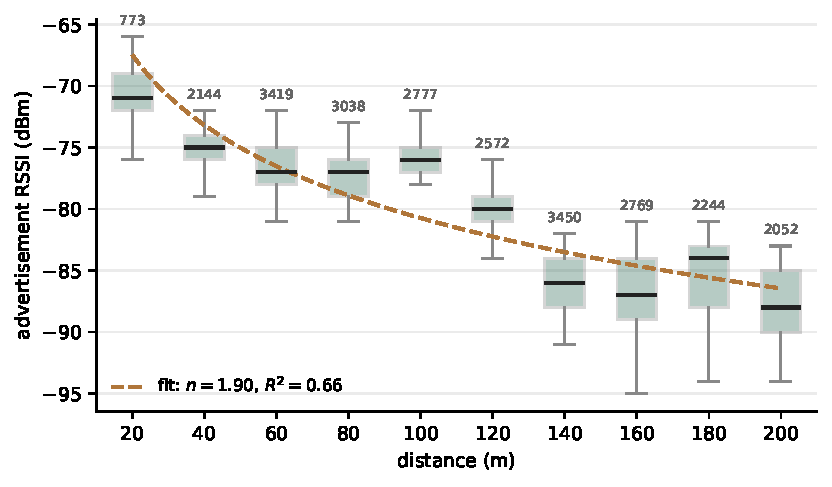
\includegraphics[width=\linewidth]{figures/line200_path_loss.pdf}
    \captionof{figure}{Path loss vs. distance}
    \column{0.42\textwidth}
    \raggeditems
    \begin{itemize}
        \item Compare to Rappaport standard path-loss model for 5G waves~\cite{Rappaport2013}
        \item Two Nexus 5X from 20 to 200\,m in 20\,m steps; ten cold-start runs per point, 100 messages each way
    \end{itemize}
    \end{columns}
    \takeaway{$\mathrm{RSSI}(d) = -43.5 - 18.8\log_{10} d$, exponent $n \approx 1.9$, residual $\sigma = 3.6$\,dB}
\end{frame}
\begin{frame}{Experiment 1, the line: time to each stage}
    \centering
    \resizebox{0.95\textwidth}{!}{%
    \begin{tikzpicture}[x=1mm,y=1mm, font=\footnotesize,
                stage/.style={draw, thick, rounded corners=1pt, fill=white, align=center, minimum height=7mm, text width=19mm, inner sep=1pt},
                tr/.style={font=\scriptsize, text=black!60, align=center, text width=21mm},
                tm/.style={font=\small\bfseries, text=TUMBlue}]
                \foreach \i/\stg/\med/\how in {
                    0/{1. Advertisement\\seen}/{1.03 s}/{scanner hears the\\peripheral},
                    1/{2. Connection\\established}/{1.55 s}/{central connects,\\MTU negotiated},
                    2/{3. Peer\\identified}/{2.39 s}/{ANNOUNCE arrives},
                    3/{4. Secure session\\established}/{2.59 s}/{Noise XX handshake\\completes},
                    4/{5. Link\\usable}/{2.70 s}/{first payload\\delivered and ACK'd}} {
                    \node[stage] (s\i) at (\i*24+10,0) {\stg};
                    \node[tm, below=0.8mm of s\i] {\med};
                    \node[tr, above=0.8mm of s\i] {\how};
                }
                \foreach \i [evaluate=\i as \j using int(\i+1)] in {0,...,3} {\draw[->, thick] (s\i) -- (s\j);}
                % \node[font=\scriptsize, text=black!60, anchor=north, align=center] at (58,-8.5) {Median time from a cold start on a Nexus 5X pair. Stage 6, \emph{link settled}: the reverse leg repeats 1--4 in parallel.};
            \end{tikzpicture}}
    \captionof{figure}{The five link stages, with median time from a cold start}
    \begin{itemize}
        \item Discovery is bound by the radio; every later stage is paid for by the application
    \end{itemize}
    \takeaway{Identifying the peer is the costliest app step at 0.84\,s, the Noise handshake adds only 0.2\,s.}
\end{frame}

\begin{frame}{Experiment 1, the line: bytes to each stage}
    \begin{columns}[T]
    \column{0.50\textwidth}
    \centering
    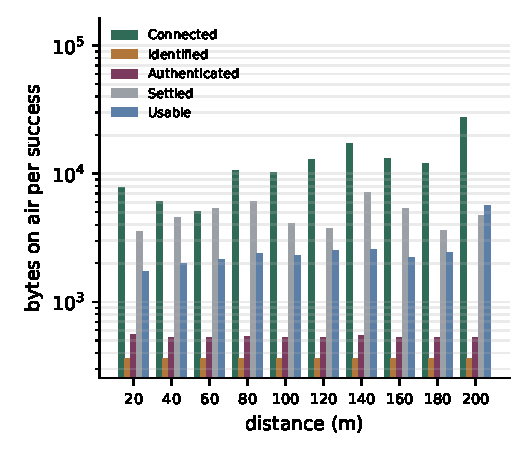
\includegraphics[width=0.96\linewidth]{figures/line200_stage_bytes_rungs.pdf}
    \captionof{figure}{Bytes to each stage, by distance}
    \column{0.50\textwidth}
    \centering
    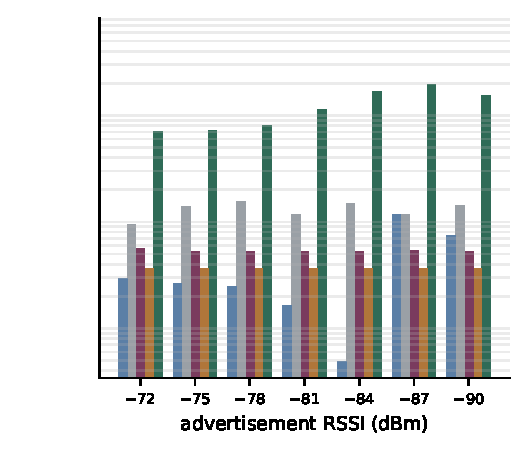
\includegraphics[width=0.96\linewidth]{figures/line200_stage_bytes_rungs_rssi.pdf}
    \captionof{figure}{The same runs, by RSSI}
    \end{columns}
    \begin{itemize}
        \item Advertising dominates the other stages: reaching a GATT link costs up to 27\,kB at a 135\,ms advertisement interval, followed by session (524 B) and identity (364 B)
        % \item Identity then costs 364\,B (two ANNOUNCEs) and a session 524\,B (four packets), both flat across RSSI
    \end{itemize}
    \takeaway{Finding the peer is what costs bytes; the secure session itself is nearly free.}
\end{frame}

\begin{frame}{Experiment 2, the diluting clique: contention collapses delivery}
    \begin{columns}[T]
    \column{0.58\textwidth}
    \centering
    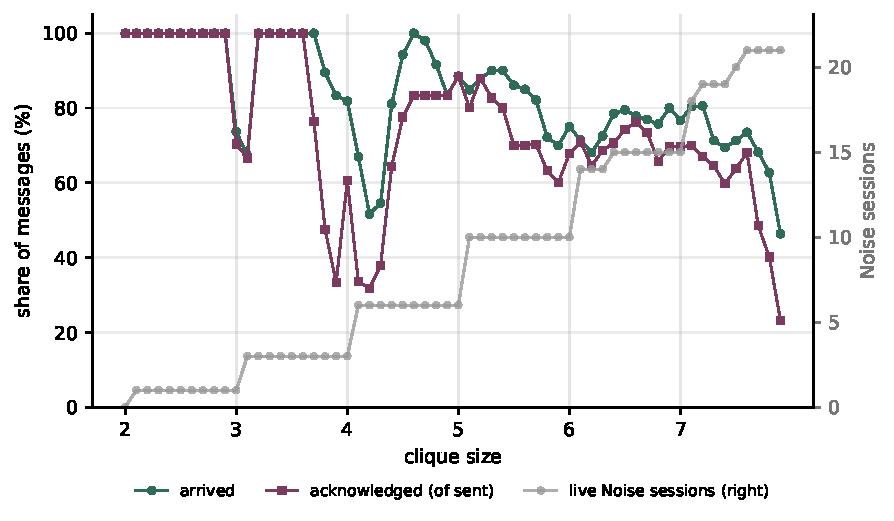
\includegraphics[width=\linewidth]{figures/clique_delivery_per_trial.pdf}
    \captionof{figure}{Delivery and ACKs per trial as the clique grows}
    \column{0.40\textwidth}
    \raggeditems
    \begin{itemize}
        \item The clique grows from 2 to 7 phones within 30\,m; offered load rises from 6.7 to 140 msg/s
        \item Delivery falls from 100\,\% to 50\,\%, ACKs to 20\,\%, median latency from 110\,ms to 9\,s
        \item Each join degrades delivery, as all nodes spend airtime on link establishment
    \end{itemize}
    \end{columns}
    \takeaway{Radio contention and hardware, not the range, are the constraints: every pair sat at a lossless RSSI.}
\end{frame}

\begin{frame}{Experiment 3, link flapping: frequent link loss, heavy-tailed outages}
    \begin{columns}[T]
    \column{0.32\textwidth}
    \centering
    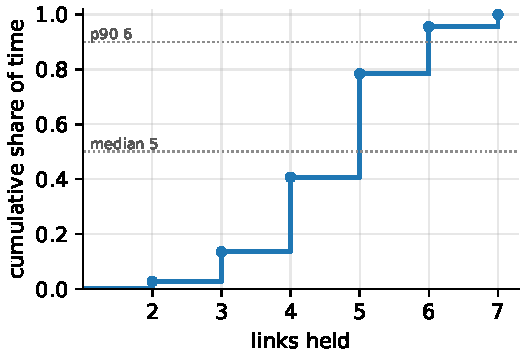
\includegraphics[height=2.6cm]{figures/churn_links_held_cdf.pdf}
    \captionof{figure}{Links held, CDF}
    \column{0.32\textwidth}
    \centering
    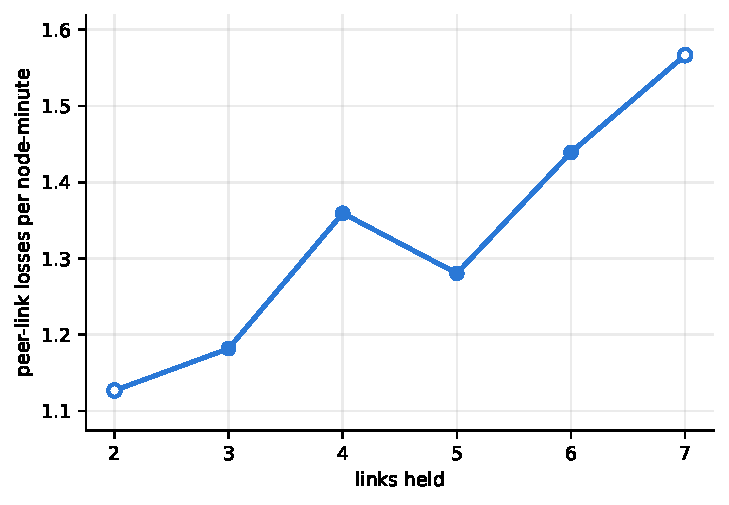
\includegraphics[height=2.6cm]{figures/churn_rate_by_degree.pdf}
    \captionof{figure}{Link loss rate vs. links held}
    \column{0.32\textwidth}
    \centering
    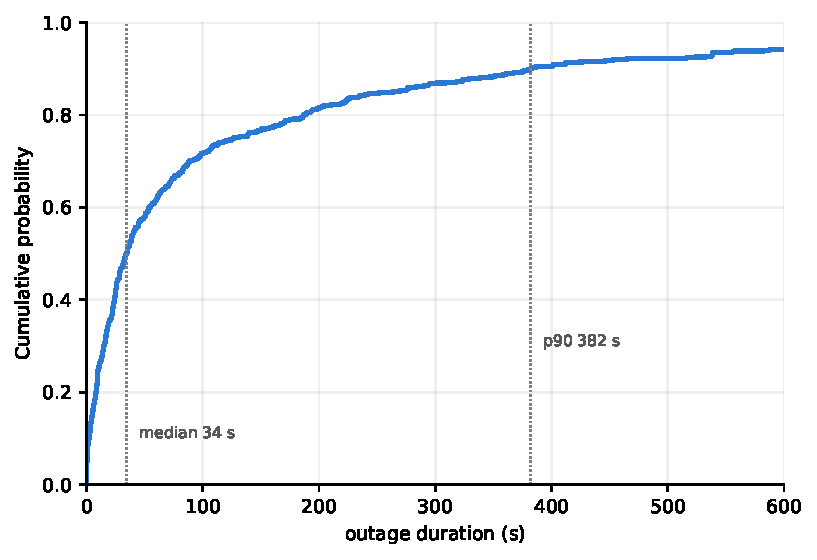
\includegraphics[height=2.6cm]{figures/churn_outage.pdf}
    \captionof{figure}{Outage duration, CDF}
    \end{columns}
    \begin{itemize}
        \item Eight phones at short range with sessions established beforehand: only physical link loss is measured
        % \item Links held by a Nexus 5X: median 5, p90 6, range 2 to 7, mean 4.7 (it sits at the 7-link cap only 4.5\,\% of the time)
        % \item Outages: median 34\,s, p90 382\,s, maximum 5\,356\,s
    \end{itemize}
    \takeaway{These distributions calibrate the simulation.}
\end{frame}

\begin{frame}{Simulations: congestion at scale}
    \begin{columns}[T]
    \column{0.44\textwidth}
    \begin{center}
        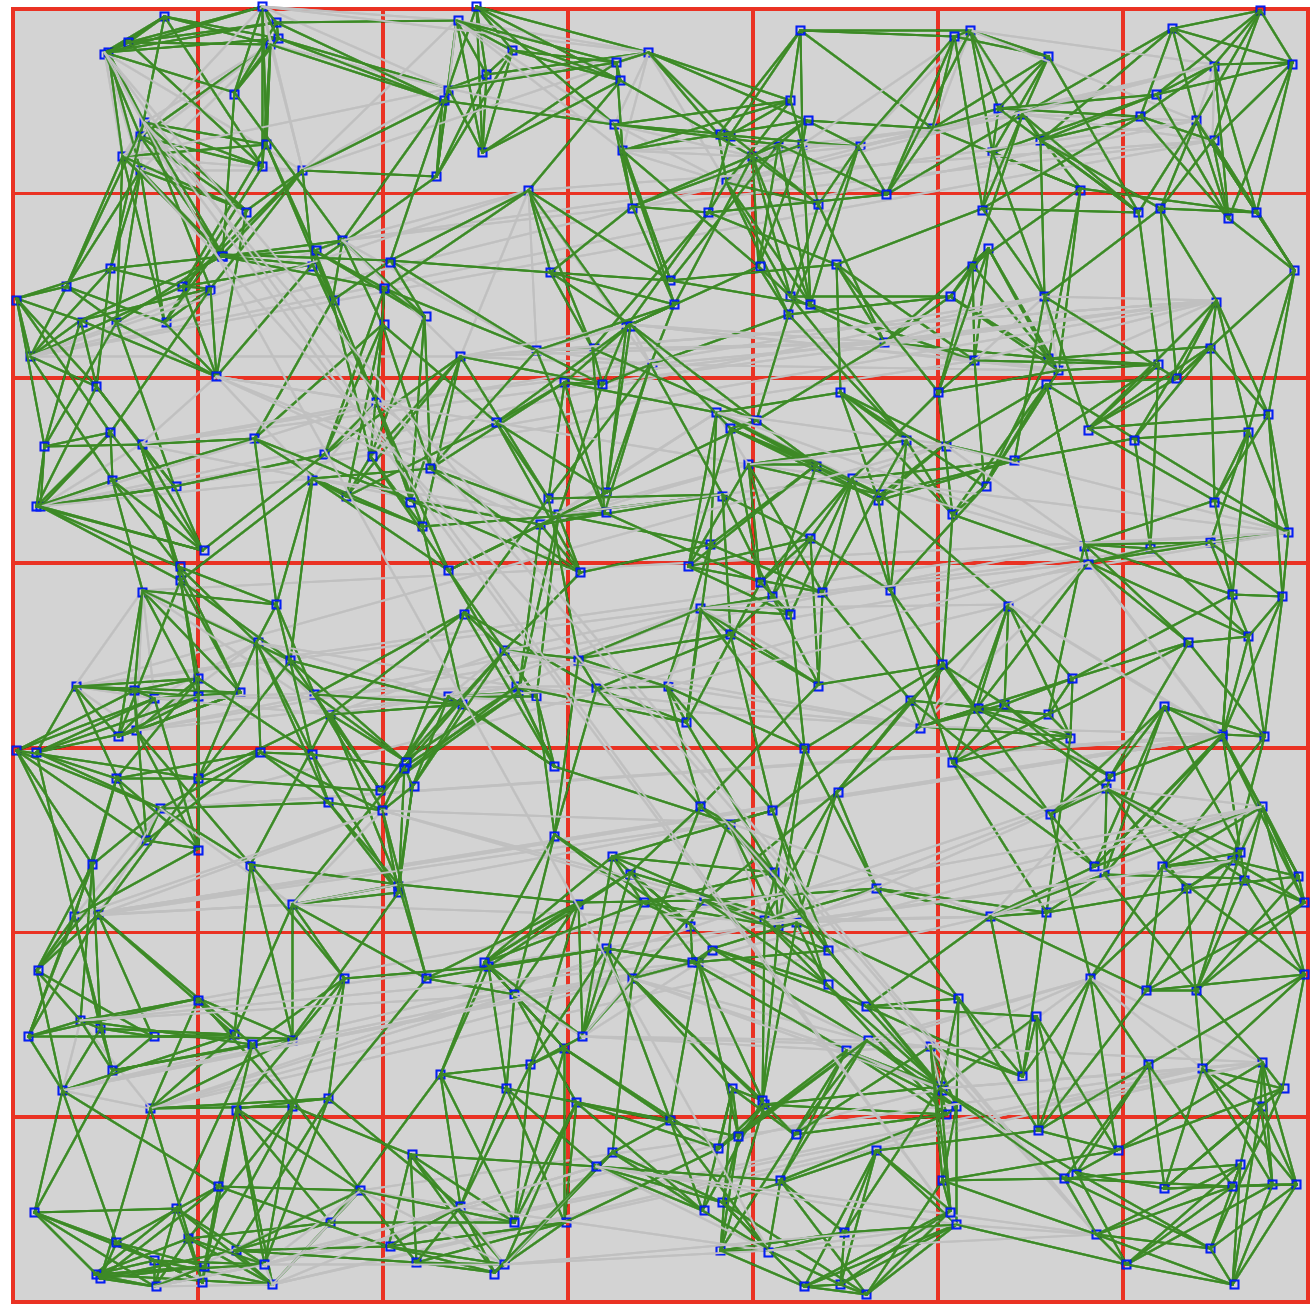
\includegraphics[width=\linewidth]{pics/sim-hall-topology.png}
    \end{center}
    \vspace{-1ex}
    {\footnotesize Red: the 49 cells of 50\,m, 8 nodes each. Green: the lanes messages flood on; grey: links held but passive}
    \column{0.54\textwidth}
    \raggeditems
    \textbf{Scenario in the ONE~\cite{the-one}}
    \begin{itemize}
        \item 350\,$\times$\,350\,m hall, 49 cells, 8 nodes per cell: 392 nodes
        \item 50\,m radio range (lossless), at most 7 links per node
        \item One new message per second for 30\,000\,s; 25 seeded placements per arm
    \end{itemize}
    \vspace{0.5ex}
    \textbf{Five control-plane establishment strategies}\\[0.5ex]
    \scriptsize
    \setlength{\tabcolsep}{4pt}
    \begin{tabular}{@{}lY{4.8cm}@{}}
        \toprule
        \texttt{flood} & epidemic flooding, as in GNL and BitChat \\
        \texttt{f3} & flood only the top 3 links by ego-network centrality~\cite{Daly2007} and buffer occupancy \\
        \texttt{oracle} & omniscient shortest path: the BLE ceiling \\
        \texttt{amigo} & leader-elected territories, after Amigo's dynamic clique routing~\cite{Inyangson2025} \\
        \texttt{amigo-udx} & \texttt{amigo} plus UDX between leaders, at the 2.4\,MB/s measured on a Nexus 5X \\
        \bottomrule
    \end{tabular}
    \end{columns}
\end{frame}

\begin{frame}{Simulations: the model the arms run on}
    % \begin{moepdef}{blue}{filled}{}
    %     \textbf{Link flapping, calibrated on experiment 3.} Every $\Delta t = 30$\,s a node $u$ holding $k_u$ links drops $D_u \sim \mathrm{Pois}\big(\lambda(k_u)\,\Delta t\big)$ of them, chosen uniformly. The measured rate depends on the links held, and the two directions differ: \emph{per node} it rises, $\lambda(k) = 1.13,\ 1.18,\ 1.36,\ 1.28,\ 1.44,\ 1.57$ per node-minute for $k = 2\ldots 7$, while \emph{per link} $\lambda(k)/k$ falls from $0.57$ to $0.22$. Endpoints draw independently, so link $i$--$j$ flaps at
    %     \[
    %         \lambda_{ij} \;=\; \frac{\lambda(k_i)}{k_i} + \frac{\lambda(k_j)}{k_j}
    %         \qquad\quad k_i = k_j = 7:\;\; \lambda_{ij} \approx 0.45\,\text{min}^{-1}, \text{ mean time between flaps 2.2 min}
    %     \]
    %     and stays down at both ends for a resampled measured outage: heavy-tailed, median $\approx$ 35\,s.
    % \end{moepdef}
    \begin{moepdef}{blue}{filled}{}
        \textbf{Link flapping, calibrated on experiment 3.} Every $\Delta t = 30$\,s a node $u$ holding $k_u$ links drops $D_u \sim \mathrm{Pois}\big(\lambda(k_u)\,\Delta t\big)$ of them, chosen uniformly. Endpoints draw independently, so link $i$--$j$ flaps at
        \[
            \lambda_{ij} \;=\; \frac{\lambda(k_i)}{k_i} + \frac{\lambda(k_j)}{k_j}
            \qquad\quad k_i = k_j = 7:\;\; \lambda_{ij} \approx 0.45\,\text{min}^{-1}, \text{ mean time between flaps 2.2 min}
        \]
        and stays down at both ends for a resampled measured outage: heavy-tailed, median $\approx$ 35\,s.
    \end{moepdef}
\end{frame}

\begin{frame}{Simulations: only the wide-area underlay overcomes the hop limit}
    \begin{center}
        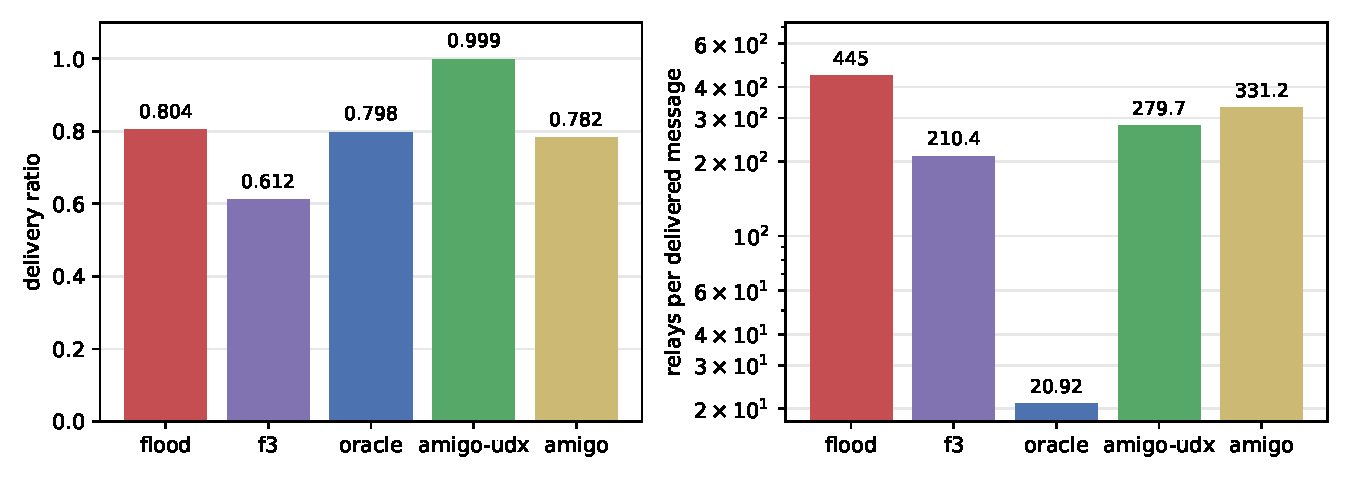
\includegraphics[width=0.86\textwidth]{figures/sim_reach_ceiling.pdf}
        \captionof{figure}{Delivery ratio and relays per delivered message, five arms}
    \end{center}
    \begin{itemize}
        \item \texttt{flood} and \texttt{oracle} both deliver about 80\,\%: the hop limit of 7 bounds reachability. Flooding costs 445 relays per delivered message, the oracle 21
        \item \texttt{f3} halves the relays but falls to 61\,\%; \texttt{amigo} on BLE alone reaches 78\,\% at near-flood cost
        \item \texttt{amigo-udx} delivers 99.9\,\% with a third fewer relays than flooding and the lowest buffer occupancy
    \end{itemize}
    \takeaway{A BLE-only mesh does not scale to this network, not even with optimal routing. Rendezvous points should be used as backbone to deliver messages across the network.}
\end{frame}

\outlineframe{5}
\section{Conclusion}
\begin{frame}{}
    \begin{moepdef}{blue}{filled}{Can BLE alone carry a grassroots social network?}
        Not at scale: delivery is bounded by the radio range under a hop limit, and by the airtime a node shares among its links.
    \end{moepdef}
    \vspace{1ex}
    % \begin{itemize}
    %     \item \textbf{Built}: GNL, one overlay over two underlays, with no servers and no relays
    %     \item \textbf{Measured} on eight smartphones: distance costs little, RSSI predicts cost, contention collapses delivery, outages are heavy-tailed
    %     \item \textbf{Simulated} at 392 nodes: BLE-only delivery saturates at 80\,\%, even with optimal routing; bridging the mesh over UDX reaches 99.9\,\%
    % \end{itemize}
    \takeaway{In a full shutdown, form links deliberately, guided by RSSI. Whenever an Internet path survives, bridge the mesh across it.}
\end{frame}

\begin{frame}{Future work}
    \begin{itemize}
        \item \textbf{Control plane}: a user-chosen scenario policy, emergency or protest, that sets link admission by RSSI and the flooding budget
        \item \textbf{Buffers}: VACCINE-style antipackets~\cite{Ott2010, Ott2011} that purge delivered messages, weighed against the presence they reveal
        \item \textbf{Handshakes}: Noise patterns for friends who already know each other's keys save a message and keep keys off the air
        \item \textbf{NAT traversal and BLE stack}: a grassroots AutoNAT through several friends; connection intervals, scan windows, stale-address failures
        \item \textbf{Beyond messaging}: opportunistic networks as a substrate for collective communication on co-located devices
    \end{itemize}
\end{frame}

\outlineframe{6}
\section{Discussion}
\begin{frame}{}
    \begin{itemize}
        \item At close range, \textbf{Contention binds the BLE mesh.} Delivery falls with the number of active links per node, at an RSSI where a single link is lossless
        \item \textbf{A second transport between rotating leaders is what scales,} from 80\,\% to 99.9\,\%. Leaders can double as gateways and rendezvous agents, and rotate as they drain
        \item \textbf{The price is exposure.} Leaders and rendezvous points attract traffic analysis and denial of service; onion-style hops would trade usability for privacy~\cite{Aceto2026}
        \item \textbf{Judge links by RSSI, not by geography,} unlike Amigo's GPS grid and CityMesh's building map~\cite{Inyangson2025, Liu2026}
        \item \textbf{Limits.} Leader election is free in the simulation; greedy linking is the wrong default in dense settings
    \end{itemize}
    \takeaway{Thank you! questions?}
\end{frame}


\section{Bibliography}
% show the citation labels used on the slides instead of beamer's icons, and set the list compactly
\setbeamertemplate{bibliography item}{\insertbiblabel}
\setbeamerfont{bibliography item}{size=\footnotesize}
\setbeamerfont{bibliography entry author}{size=\footnotesize}
\setbeamerfont{bibliography entry title}{size=\footnotesize}
\setbeamerfont{bibliography entry location}{size=\footnotesize}
\setbeamerfont{bibliography entry note}{size=\footnotesize}
\begin{frame}[allowframebreaks]
    \footnotesize
    \setlength{\itemsep}{0pt}
    \bibliographystyle{firstauthorYY}
    \bibliography{references}
\end{frame}

\section{Backup}
\begin{frame}{Experiment 1, the line: RSSI, not distance, predicts the cost}
    \begin{columns}[T]
    \column{0.48\textwidth}
    \centering
    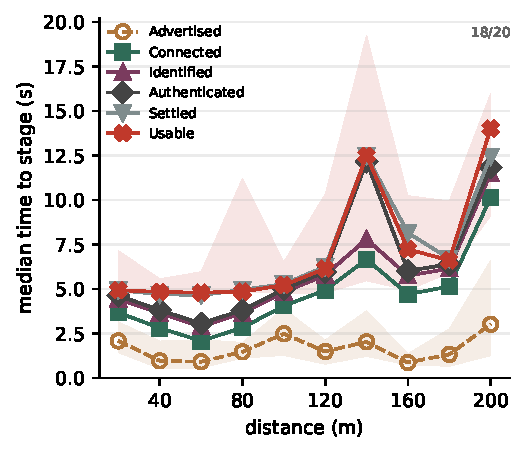
\includegraphics[width=\linewidth]{figures/line200_stages.pdf}
    \captionof{figure}{Time to link stage, by distance}
    \column{0.48\textwidth}
    \centering
    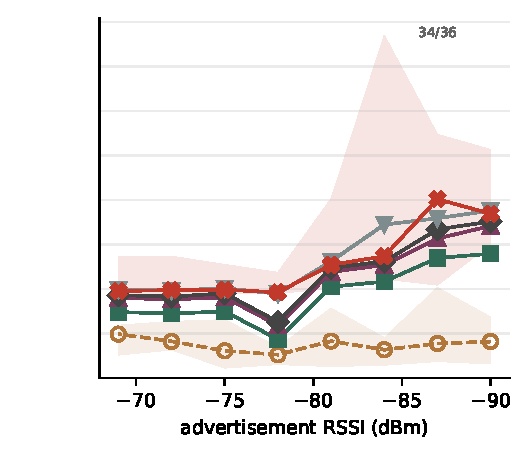
\includegraphics[width=\linewidth]{figures/line200_stages_vs_rssi.pdf}
    \captionof{figure}{The same runs, by RSSI}
    \end{columns}
    \begin{itemize}
        \item Discovery is quick and bound by the radio; identifying the peer is what costs. % 99 of 100 runs reached a session
        \item By distance the picture is confusing: RSSI values measured at different distances overlap
    \end{itemize}
    \takeaway{Pooled by RSSI, every stage rises monotonically.}
\end{frame}
\begin{frame}{Experiment 1, the line: delivery and acknowledgements}
    \begin{columns}[T]
    \column{0.48\textwidth}
    \centering
    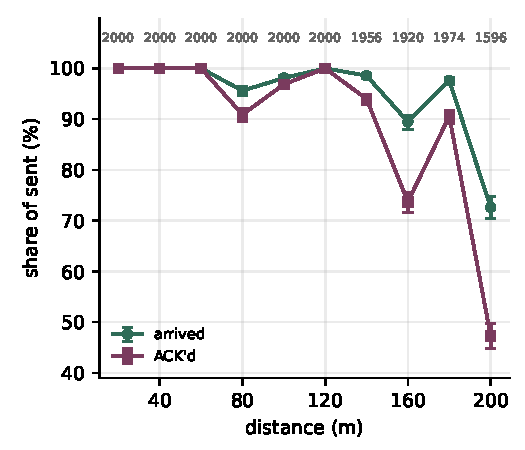
\includegraphics[width=\linewidth]{figures/line200_delivery_vs_distance.pdf}
    \captionof{figure}{Delivery and ACKs, by distance}
    \column{0.48\textwidth}
    \centering
    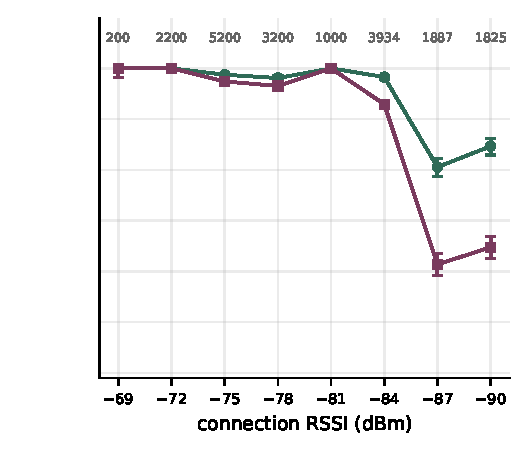
\includegraphics[width=\linewidth]{figures/line200_delivery_vs_rssi.pdf}
    \captionof{figure}{The same runs, by RSSI}
    \end{columns}
    \begin{itemize}
        \item Lossless above $-84$\,dBm%; beyond 120\,m the median ACK time climbs from 150\,ms to 3.1\,s
    \end{itemize}
    \takeaway{Judge links by RSSI.}
\end{frame}
\begin{frame}{Experiment 2, the diluting clique: custody does not rescue delivery}
    \begin{columns}[T]
    \column{0.56\textwidth}
    \centering
    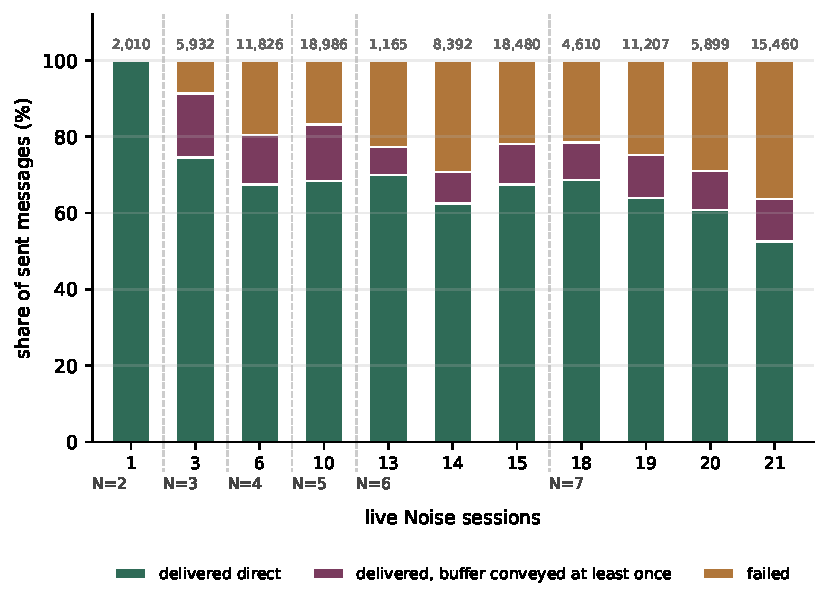
\includegraphics[width=\linewidth]{figures/clique_delivery_outcome_by_sessions.pdf}
    \captionof{figure}{Per-message outcome by live Noise sessions}
    \column{0.42\textwidth}
    \raggeditems
    \begin{itemize}
        \item Per message: delivered directly, conveyed from a peer's buffer, or failed
        \item Direct delivery drops to about 50\,\% at 21 live sessions; failures rise from 9\,\% to 37\,\%
        \item Conveyance covers only 5 to 10\,\% of deliveries
    \end{itemize}
    \end{columns}
    \takeaway{Greedy link establishment fails under contention: control plane link establishment needs a strategy.}
\end{frame}

\begin{frame}{Expriment3 the link-flap model in numbers}
    \begin{columns}[T]
    \column{0.52\textwidth}
    \centering
    \textbf{Nexus 5X link losses used by the simulator}\\[0.5ex]
    \small
    \begin{tabular}{@{}rrr@{}}
        \toprule
        links held $k$ & $\lambda(k)$ per node-minute & per link, $\lambda(k)/k$ \\
        \midrule
        1 & 1.13 & 1.13 \\
        2 & 1.13 & 0.57 \\
        3 & 1.18 & 0.39 \\
        4 & 1.36 & 0.34 \\
        5 & 1.28 & 0.26 \\
        6 & 1.44 & 0.24 \\
        7 & 1.57 & 0.22 \\
        \bottomrule
    \end{tabular}\\[1ex]
    {\footnotesize $k = 1$ was never observed and reuses the value of $k = 2$}
    \column{0.46\textwidth}
    \raggeditems
    \begin{itemize}
        \item The per-node rate rises mildly with $k$, while the per-link rate falls: a node with more links is not proportionally more fragile per link
        \item Every 30\,s each node draws a Poisson number of drops and picks the victim links uniformly
        \item Outage lengths are resampled from 1\,000 quantiles of the measured Nexus 5X outages: median 37\,s, mean 236\,s, maximum 5\,356\,s
        \item An exponential fit was rejected: too few short and too few very long outages
    \end{itemize}
    \end{columns}
\end{frame}

% \begin{frame}{Path loss along the line}
%     \centering
%     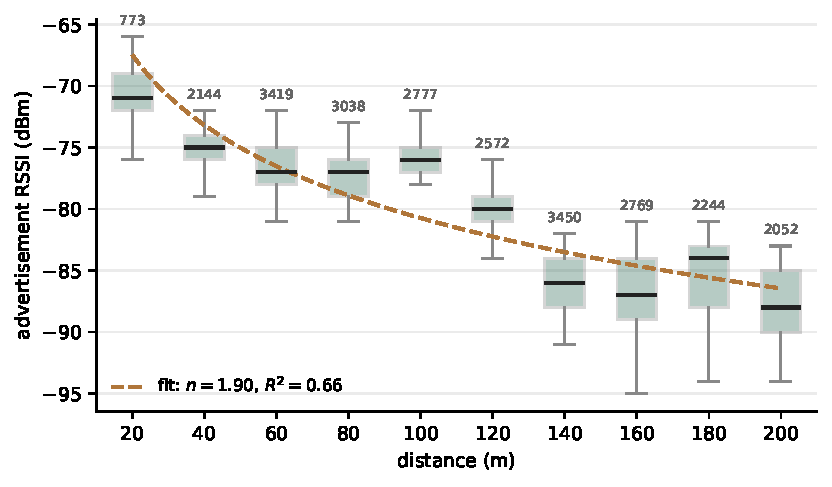
\includegraphics[width=0.66\textwidth]{figures/line200_path_loss.pdf}
%     \captionof{figure}{$\mathrm{RSSI}(d) \approx -43.5 - 18.8\log_{10} d$, a path-loss exponent of about 1.9, residual $\sigma = 3.6$\,dB, fitted on 34\,669 advertisement sightings at ten positions}
% \end{frame}

% \begin{frame}{Time to link stage by distance}
%     \begin{columns}[T]
%     \column{0.48\textwidth}
%     \centering
%     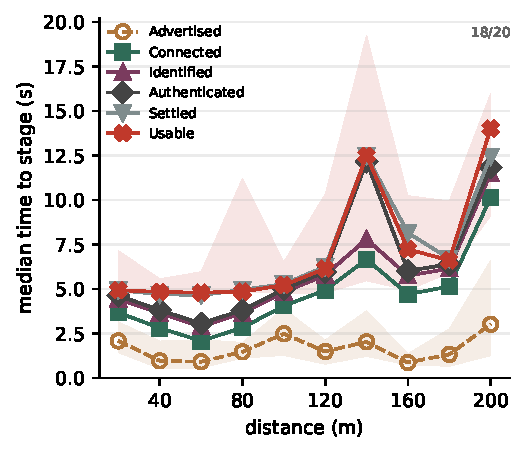
\includegraphics[width=\linewidth]{figures/line200_stages.pdf}
%     \captionof{figure}{Time to each link stage, by distance}
%     \column{0.5\textwidth}
%     \centering
%     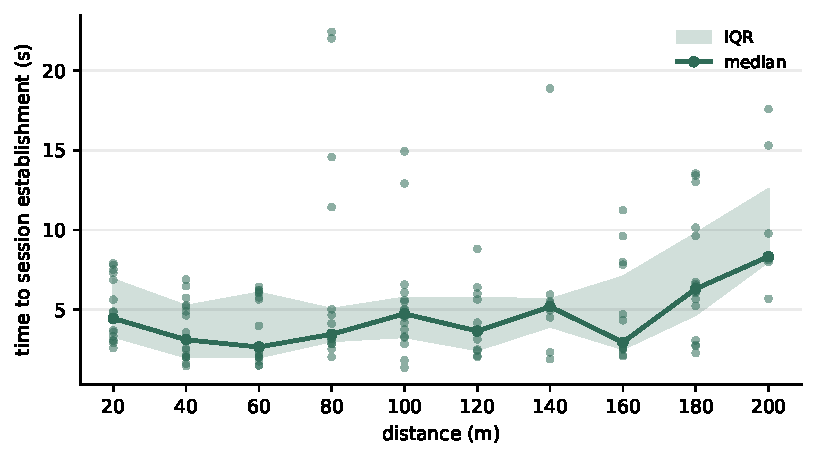
\includegraphics[width=\linewidth]{figures/line200_establishment_clean.pdf}
%     \captionof{figure}{Time to session, runs with GATT dial errors removed}
%     \end{columns}
%     \begin{itemize}
%         \item Hardware errors in the Bluetooth stack, especially around 140\,m, dominate the raw medians; removing those runs gives the expected upward trend
%     \end{itemize}
% \end{frame}

\begin{frame}{Delivery under load along the line}
    \centering
    \small
    \begin{tabular}{@{}rrrrrrr@{}}
        \toprule
        \textbf{d (m)} & \textbf{sent} & \textbf{arrived} & \textbf{acked} & \textbf{arrived} & \textbf{acked} & \textbf{ack p50} \\
        \midrule
         20 & 2000 & 2000 & 2000 & 100.0\,\% & 100.0\,\% &  123\,ms \\
         40 & 2000 & 2000 & 2000 & 100.0\,\% & 100.0\,\% &  133\,ms \\
         60 & 2000 & 2000 & 2000 & 100.0\,\% & 100.0\,\% &  135\,ms \\
         80 & 2000 & 1912 & 1818 &  95.6\,\% &  95.1\,\% &  150\,ms \\
        100 & 2000 & 1962 & 1937 &  98.1\,\% &  98.7\,\% &  144\,ms \\
        120 & 2000 & 2000 & 2000 & 100.0\,\% & 100.0\,\% &  166\,ms \\
        140 & 1956 & 1928 & 1838 &  98.6\,\% &  95.3\,\% &  380\,ms \\
        160 & 1920 & 1719 & 1415 &  89.5\,\% &  82.3\,\% & 1919\,ms \\
        180 & 1974 & 1929 & 1788 &  97.7\,\% &  92.7\,\% &  435\,ms \\
        200 & 1596 & 1161 &  755 &  72.7\,\% &  65.0\,\% & 3138\,ms \\
        \midrule
        all & 19446 & 18611 & 17551 & 95.7\,\% & 94.3\,\% & 154\,ms \\
        \bottomrule
    \end{tabular}\\[1ex]
    {\footnotesize 100 messages per trial per direction, both directions pooled; ack latency is the per-trial median of medians}
\end{frame}

% \begin{frame}{Control-plane bytes to reach each link stage}
%     \begin{columns}[T]
%     \column{0.42\textwidth}
%     \centering
%     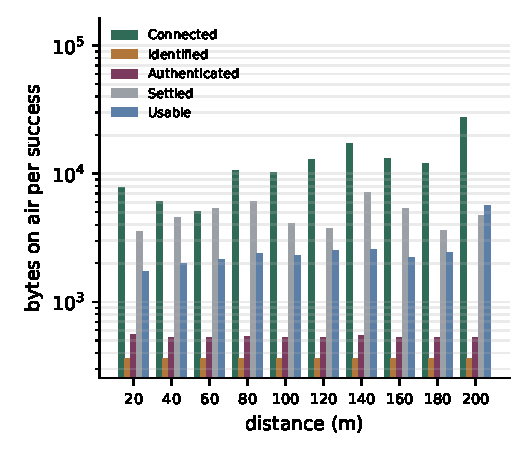
\includegraphics[width=\linewidth]{figures/line200_stage_bytes_rungs.pdf}
%     \captionof{figure}{Bytes to each link stage, by distance}
%     \column{0.42\textwidth}
%     \centering
%     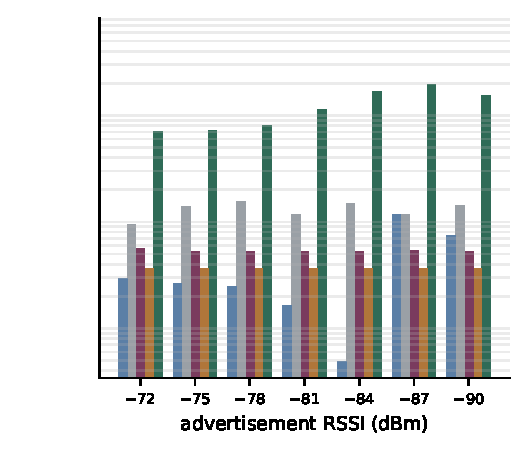
\includegraphics[width=\linewidth]{figures/line200_stage_bytes_rungs_rssi.pdf}
%     \captionof{figure}{Bytes to each link stage, by RSSI}
%     \end{columns}
%     \begin{itemize}
%         \item Establishing a GATT link costs 5 to 27\,kB of advertising at a 135\,ms interval
%         \item Identity costs 364 B (two ANNOUNCEs) and a session 524 B (four packets), whatever the RSSI
%     \end{itemize}
% \end{frame}

\begin{frame}{Delivery and latency along the line, by distance}
    \centering
    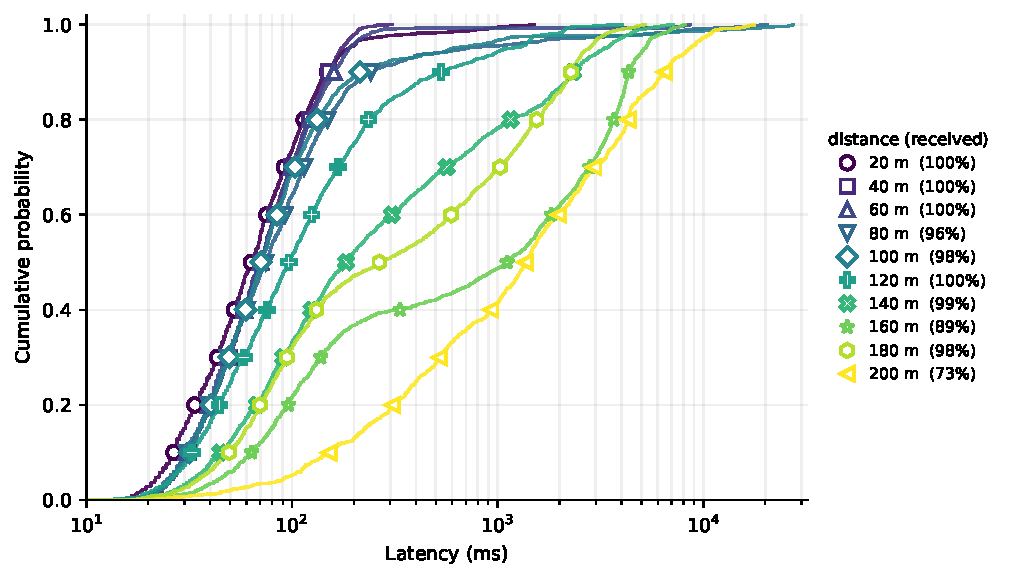
\includegraphics[width=\linewidth]{figures/line200_latency_cdf.pdf}
    \captionof{figure}{Message latency CDF, by distance}
\end{frame}

\begin{frame}{The diluting clique in numbers}
    \centering
    \small
    \setlength{\tabcolsep}{2.5pt}
    \begin{tabular}{@{}rrrrrrr@{}}
        \toprule
        \textbf{N} & \textbf{offered} & \textbf{sent} & \textbf{arrived} & \textbf{acked} & \textbf{lat p50} & \textbf{carried} \\
        \midrule
        2 &   6.7/s &  2000 & 100.0\,\% & 100.0\,\% & 0.11\,s &  0.0\,\% \\
        3 &  20.0/s &  5965 &  91.5\,\% &  79.5\,\% & 11.0\,s &  5.4\,\% \\
        4 &  40.0/s & 11940 &  80.3\,\% &  63.9\,\% & 31.6\,s & 10.1\,\% \\
        5 &  66.7/s & 19736 &  83.6\,\% &  75.1\,\% & 12.3\,s &  7.6\,\% \\
        6 & 100.0/s & 28793 &  75.7\,\% &  70.3\,\% &  8.3\,s &  6.5\,\% \\
        7 & 140.0/s & 38112 &  70.3\,\% &  57.8\,\% &  9.1\,s & 10.4\,\% \\
        \bottomrule
    \end{tabular}

    \vspace{1ex}
    {\footnotesize Ten trials per clique size, pooled over all senders; offered load in messages per second. \emph{Carried}: share of deliveries made out of a store-carry-forward buffer rather than over a live link.}
\end{frame}

\begin{frame}{Advertising cadence at idle}
    \centering
    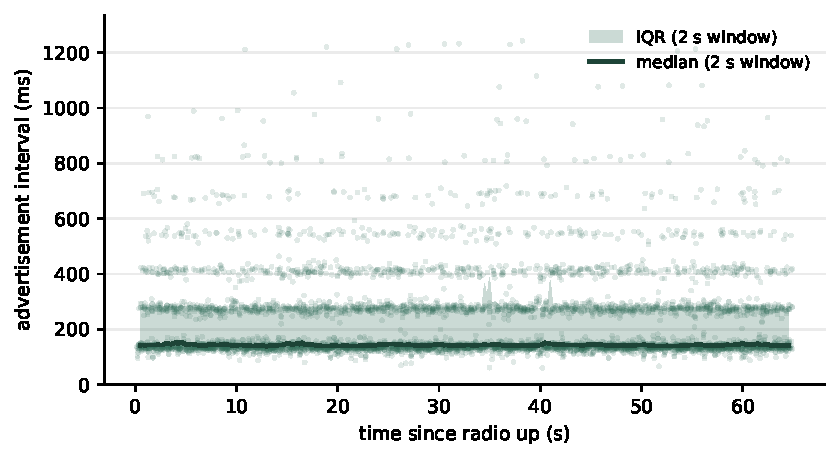
\includegraphics[width=0.8\textwidth]{figures/adv_interval_idle.pdf}
    \captionof{figure}{Median 7.41\,Hz, an advertisement interval of about 135\,ms, over twenty cold desk runs; even with an idle scanner roughly a third of the advertisements are not captured. Native stacks expose no callback for sent advertisements, so this baseline estimates the advertising bytes on the line.}
\end{frame}

\begin{frame}{Raw capacity of the two underlays on a Nexus 5X}
    \begin{columns}[T]
    \column{0.48\textwidth}
    \centering
    \textbf{BLE, one GATT link, 1\,m, write without response}\\[0.5ex]
    \small
    \begin{tabular}{@{}rrr@{}}
        \toprule
        Write size (B) & Writes/s & Delivered (kB/s) \\
        \midrule
        64  & 202 & 12.9 \\
        138 & 222 & 30.7 \\
        244 & 223 & 54.5 \\
        380 & 165 & 62.7 \\
        448 & 145 & 65.0 \\
        514 & 125 & 64.1 \\
        \bottomrule
    \end{tabular}\\[1ex]
    {\footnotesize The binding constraint is writes per second, not bytes offered; the ceiling is 63 to 65\,kB/s at the full 514-byte ATT payload}
    \column{0.48\textwidth}
    \centering
    \textbf{UDX, one isolate per stream}\\[0.5ex]
    \small
    \begin{tabular}{@{}rr@{}}
        \toprule
        Concurrent peers & Total throughput (bytes/s) \\
        \midrule
        1  & 628\,800 \\
        2  & 1\,321\,300 \\
        4  & 1\,952\,600 \\
        6  & 1\,634\,900 \\
        20 & 2\,459\,200 \\
        48 & 2\,406\,300 \\
        96 & 1\,757\,500 \\
        \bottomrule
    \end{tabular}\\[1ex]
    {\footnotesize About 2.4\,MB/s, the UDX capacity used by the \texttt{amigo-udx} arm}
    \end{columns}
\end{frame}

\begin{frame}{Buffer occupancy at scale}
    \centering
    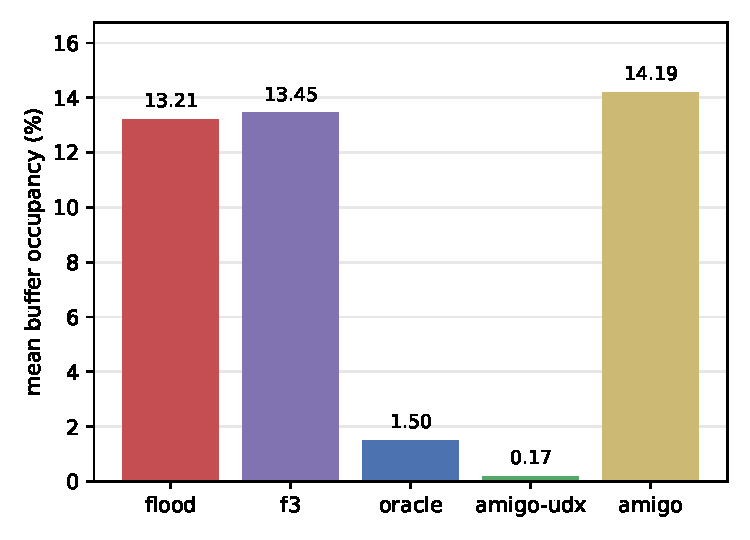
\includegraphics[width=0.66\textwidth]{figures/sim_buffer_occupancy.pdf}
    \captionof{figure}{Mean DTN buffer occupancy for the five arms at 392 nodes, 1\,msg/s network-wide, 25 seeded placements per arm. \texttt{amigo-udx} needs the least buffer; \texttt{f3} relays half as much as \texttt{flood} but buffers the same; \texttt{amigo} over BLE alone buffers the most.}
\end{frame}

\begin{frame}{Noise XX in three messages}
    \centering
    \begin{tikzpicture}[x=1mm,y=1mm, font=\small,
        note/.style={font=\footnotesize, text=black!65, text width=30mm},
        msg/.style={->, thick, TUMBlue}]
        \node[font=\small\bfseries] at (36,50) {Initiator $i$};
        \node[font=\small\bfseries] at (82,50) {Responder $r$};
        \draw[thick, black!60] (36,47) -- (36,2);
        \draw[thick, black!60] (82,47) -- (82,2);
        \draw[msg] (36,42) -- (82,40) node[midway, above=1.5pt, sloped] {1: \texttt{e}, cleartext, 115 B};
        \draw[msg] (82,29) -- (36,27) node[midway, above=1.5pt, sloped] {2: \texttt{e, ee, s, es}, 163 B};
        \draw[msg] (36,16) -- (82,14) node[midway, above=1.5pt, sloped] {3: \texttt{s, se}, 131 B};
        \node[note, anchor=east, align=right] at (34,42) {fresh ephemeral key $e_i$};
        \node[note, anchor=west, align=left] at (84,34) {fresh $e_r$; derive \texttt{ee}, \texttt{es}; send the static key $s_r$ encrypted};
        \node[note, anchor=east, align=right] at (34,21) {decrypt $s_r$, abort unless it equals the announced key; encrypt $s_i$, derive \texttt{se}};
        \node[note, anchor=west, align=left] at (84,9) {decrypt $s_i$, abort unless it equals the announced key};
        \node[note, anchor=east, align=right] at (34,5) {\texttt{Split()}: two transport ciphers};
        \node[note, anchor=west, align=left] at (84,1) {\texttt{Split()}: two transport ciphers};
    \end{tikzpicture}
    \captionof{figure}{\texttt{e}: send a fresh ephemeral key. \texttt{s}: send the static key. \texttt{ee}, \texttt{es}, \texttt{se}: Diffie-Hellman between the named keys, mixed into the chaining key with HKDF. Both peers send message 1; the lexicographically lower public key takes the responder role.}
\end{frame}

\begin{frame}{Wire format}
    \begin{columns}[T]
    \column{0.48\textwidth}
    \centering
    \textbf{ANNOUNCE payload}\\[1ex]
    \begin{bytefield}[bitwidth=0.5em, bitheight=3.2ex, bitformatting={\tiny}, boxformatting={\centering\scriptsize}]{32}
        \bitheader{0,8,16,24,31} \\
        \offset{0}\bitbox{32}{Public key (32 B)} \\
        \offset{32}\bitbox{8}{Flags} \bitbox{8}{Nick len} \bitbox{16}{Candidate count} \\
        \offset{36}\wordbox[tlr]{1}{Nickname (variable)} \\
        \wordbox[tlr]{1}{Repeated IP candidates (variable)} \\
        \wordbox[tlr]{1}{Signature (64 B)}
    \end{bytefield}\\[1ex]
    {\footnotesize Sent in cleartext with TTL 1; signed by the creator}
    \column{0.48\textwidth}
    \centering
    \textbf{GrassrootsPacket header, 60 B}\\[1ex]
    \begin{bytefield}[bitwidth=0.5em, bitheight=3.2ex, bitformatting={\tiny}, boxformatting={\centering\scriptsize}]{32}
        \bitheader{0,8,16,24,31} \\
        \offset{0}\bitbox{8}{Type} \bitbox{8}{TTL} \bitbox{16}{Recipient} \\
        \offset{4}\wordbox[tlr]{1}{Recipient, continued (32 B in total)} \\
        \offset{34}\bitbox{16}{Recipient} \bitbox{16}{Packet ID} \\
        \wordbox[tlr]{1}{Packet ID, continued (16 B in total)} \\
        \offset{50}\bitbox{16}{Packet ID} \bitbox{16}{Length} \\
        \offset{54}\bitbox{16}{Length} \bitbox{16}{Payload} \\
        \wordbox[tlr]{1}{Payload (variable)}
    \end{bytefield}\\[1ex]
    {\footnotesize No sender, no signature: the Noise session authenticates the sender; the recipient field avoids trial decryption of transit packets}
    \end{columns}
\end{frame}

\begin{frame}{Crypto testbench: the cost of trial decryption}
    \begin{center}
    \begin{tabular}{@{}rrrr@{}}
        \toprule
        active sessions & per transit packet & packets/s to saturate one core & CPU at 10 packets/s \\
        \midrule
        8 & 2.93\,ms & 341 & 2.9\,\% \\
        32 & 11.5\,ms & 87 & 11.5\,\% \\
        128 & 44.8\,ms & \textbf{22} & 44.8\,\% \\
        \bottomrule
    \end{tabular}
    \end{center}
    \vspace{1ex}
    \begin{itemize}
        \item Measured on a Nexus 5X: trial decryption of one transit packet against a growing number of active Noise sessions
        \item The header carries no sender, so the receiver finds it by trial decryption, most recently used session first
        \item Without a recipient field every transit packet would pay this cost: an active user with 128 sessions saturates one core at 22 packets per second, and spends almost half a core at only 10
        \item Hence the header keeps the recipient and omits the sender
    \end{itemize}
\end{frame}

\begin{frame}{Testbed hardware}
    \begin{center}
    \begin{tabular}{@{}cclllc@{}}
        \toprule
        Units & Join order & Device & SoC & OS & Bluetooth \\
        \midrule
        4 & 1--4 & LG Nexus 5X & Snapdragon 808 & Android 8.1 & 4.2 \\
        2 & 5--6 & Google Pixel 10 Pro & Tensor G5 & Android 16 & 6.0 \\
        1 & 7 & Samsung Galaxy S10e & Exynos 9820 & Android 12 & 5.0 \\
        1 & 8 & Huawei HMA-L09 & Kirin 960 & Android 9 & 4.2 \\
        \bottomrule
    \end{tabular}
    \end{center}
    \vspace{1ex}
    \begin{itemize}
        \item All phones stand on tripods outdoors and interoperate at Bluetooth 4.2
        \item The join order is the order in which devices enter the diluting clique
        \item The Huawei is the eighth device, used in the link flapping experiment
    \end{itemize}
\end{frame}

\end{document}
